% !TeX root = Logpp.tex
This section describes opportunities, using language, runtime, or compiler support, to address 
general challenges surrounding logging outlined in \autoref{sec:intro}. We can roughly divide 
these into two classes -- performance oriented and functionality oriented. 

\subsection{Logging Performance}
\label{subsec:performancedesign}

\begin{design}
The cost of a logging statement at a logging level that 
is disabled should have zero-cost at runtime. This includes both the direct 
cost of the logging action and the indirect cost of of building a format 
string and processing any arguments. Further, disabling/enabling a log 
statement should not change the semantics the application.
\end{design}

When logging frameworks are included as libraries the compiler/JIT does not, 
in general, have any deep understanding of the enabled/disabled semantics of 
the logger. As a result the compiler/JIT will not be able to fully eliminate 
dead-code associated with disabled logging statements and will incur, individually 
small but widespread, parasitic costs for each disabled logging statement. 
These costs can be very difficult to diagnose, as they are widely dispersed and 
individually small, but can add up to several percentage points of application 
runtime. To avoid these parasitic costs we propose including logging primitives 
in the core specification of the programming language or, if that is not possible, 
adding compiler/JIT specializations to optimize them. 

An additional advantage of lifting log semantics to the language specification 
level is the ability to statically verify logging uses and handle errors that 
occur during log expression evaluation. Common errors include 
format specifier violations~\cite{tyepcheckprintf}, accidental state 
modification~\cite{mypurity,choipurity} in the logging message computation, and other logging anti-patterns~\cite{logginganti}. 
If the language semantics 
specify logging API's then both of these error classes can be statically 
checked to avoid runtime errors or heisenbugs that appear/disappear when logging 
levels are changed.

\begin{design}
The cost of an enabled logging statement has two components -- (1) the cost to 
compute the set of arguments to the log statement and (2) the cost to format and 
write this data into the log. The cost of computing the argument values is, in 
general unavoidable, and must be done on the hot path of execution. However, 
the cost of (2) should be reduced and/or moved off the hot path as much as possible.
\end{design}

To minimize the cost of computing arguments to the log statement and speed their 
processing we propose a novel log format specification mechanism using 
\emph{preprocessed} and stored log formats along with a set of \emph{log expandos} 
which can be used as a shorthand in a log to specify common, but expensive/complicated, 
to compute log argument values. The use of preprocessed format messages allows us to save time, 
the type checking and processing of each argument does not require parsing the 
format string, and instead of eagerly stringifying each parameter we can do a quick 
immutable copy of the argument which can be formatted later. Expandos provide convenient 
ways to add data into the log, such as the current date/time, the host IP, or a 
current request ID~\cite{asynchjs}, that would either be more expensive or more awkward to compute 
explicitly on a regular basis. We can eliminate the main-thread cost of formatting by batching 
the log messages and instead doing the format work on a background task thread.

\begin{figure*}
    \centering
    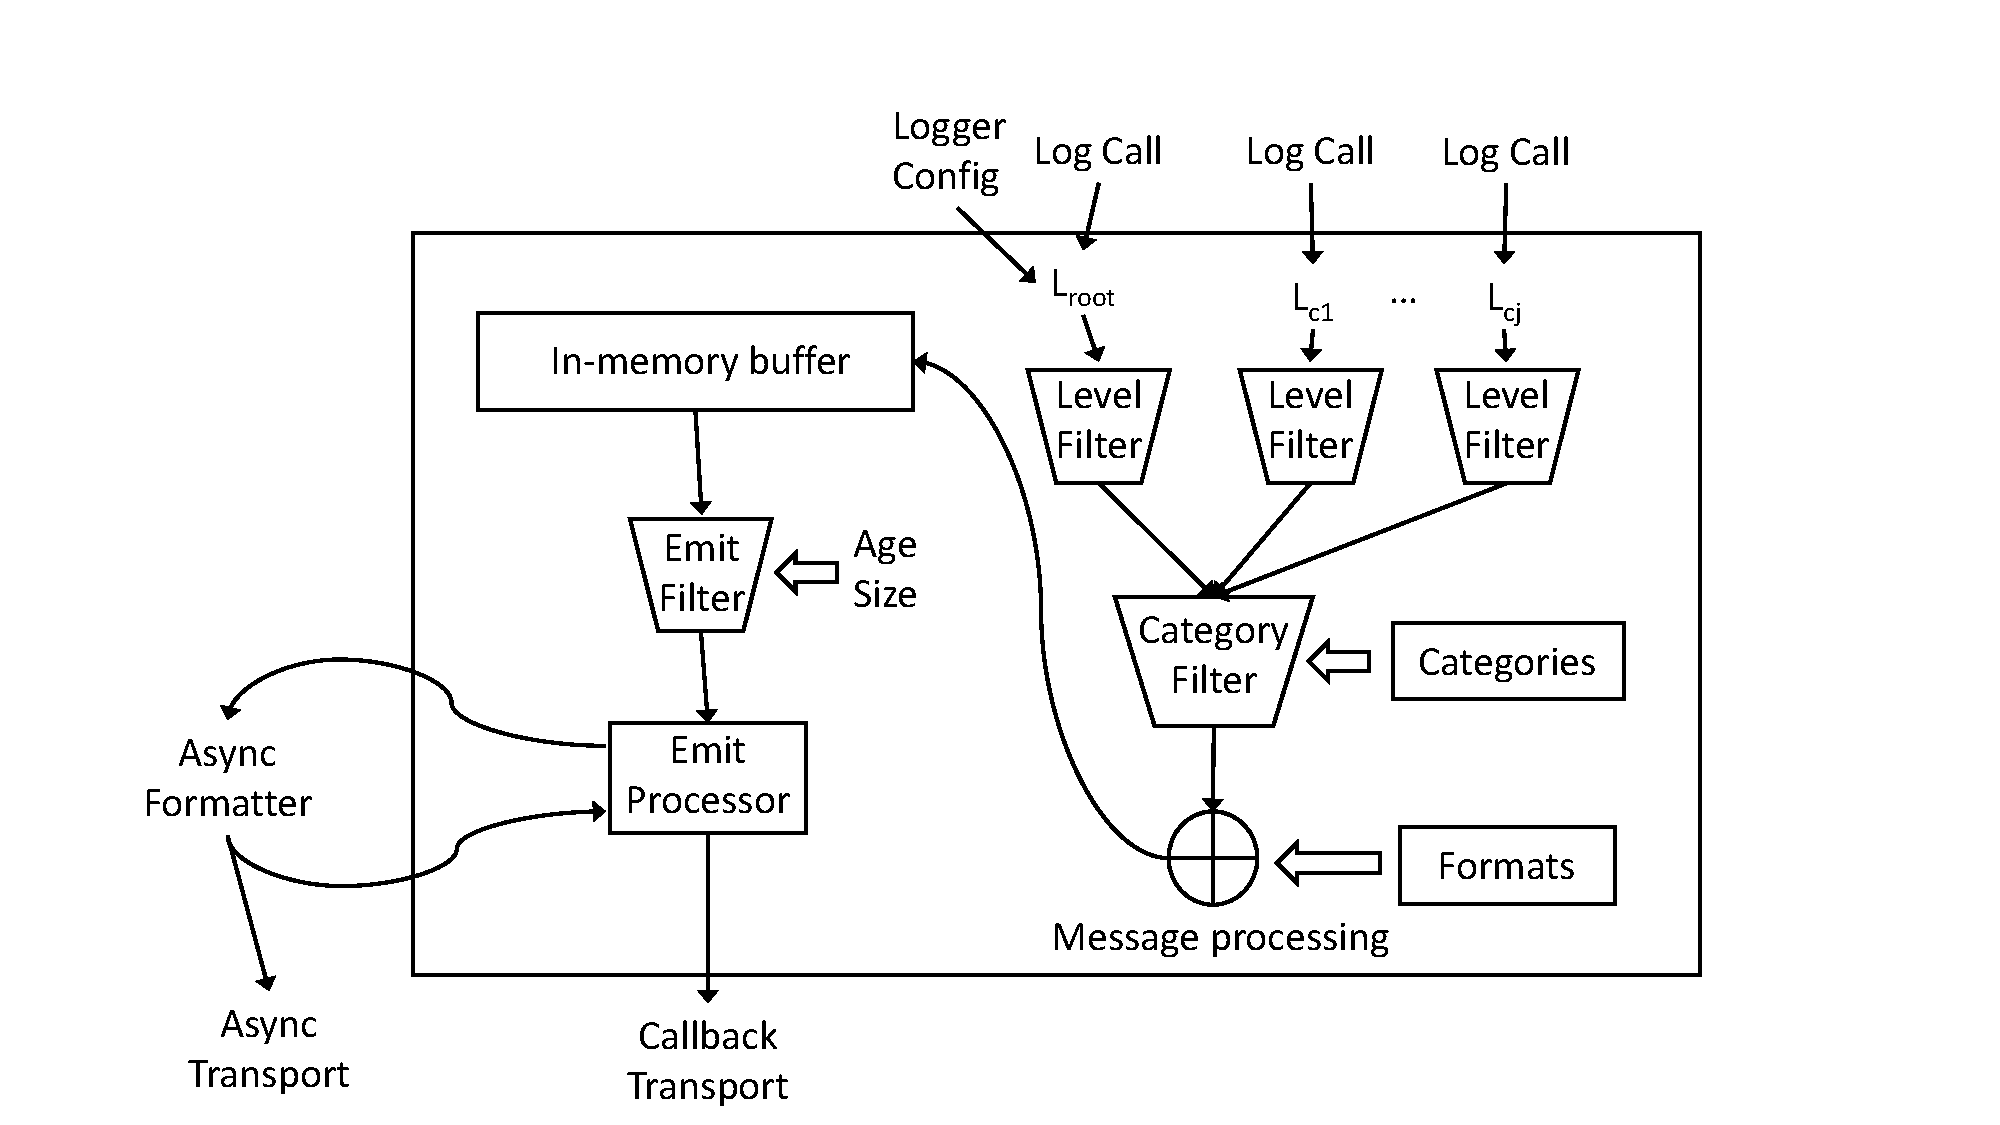
\includegraphics[width=0.8\textwidth]{Figures/ArchDiagram}
    \caption{Logger architecture}
    \label{fig:arch}
\end{figure*}

\subsection{Logging Functionality}
\label{subsec:functionalitydesign}
\begin{design}
Logging serves two related, but somewhat conflicting roles, in modern systems. 
The first role is to provide detailed information 
on the sequence of events preceding a bug to aid the developer in triaging and 
reproducing the issue. The second role is to provide general telemetry 
information and visibility into the overall behavior of the application. 
This observation leads to the third design principle: logging should 
support both tasks simultaneously without compromising the 
effectiveness of either one.
\end{design}

To support these distinct roles we propose a dual-level logging approach. In the 
first level all messages are initially stored, as a format + immutable 
arguments, into an in-memory buffer. This operation is high performance and 
suitable for high frequency writes of detailed logging information needed for 
debugging. Further, in event an error is encountered the full contents of 
detailed logging can be flushed to aid in debugging. In the second level these 
detailed messages can be filtered out and only the high-level telemetry focused 
messages can be saved, formatted, and written into the stable log. This filtering 
avoids the pollution the saved logs with overly detailed information while 
preserving the needed data for monitoring the overall status of the application~\cite{logstudy,logstudy2}. 

\begin{design}
Logging code should not obscure the logic of the application that it is 
supporting. Thus, a logger should provide specialized logging primitives 
that cover common cases, such as conditional logging, that would otherwise 
require a developer to add new logic flow into their application specifically 
for logging purposes.
\end{design}

Common scenarios that often involve additional control or data flow logic 
include \emph{conditional logging} where a message is only written when a 
specific condition is satisfied, \emph{child loggers} which handle a specific 
subtask and often developers want to include additional information in all 
log messages from this subtask, and \emph{bracketing entries} where 
developers want to mark the start/end of something and include correlated 
timing (and other) information in the bracketing. All of these scenarios 
involve the developer adding additional, error-prone, control and data flow 
to the program which obscures the core algorithmic code. Thus, we propose 
adding primitive methods for supporting all of these scenarios without requiring 
additional developer implemented logic.

\begin{design}
Applications are often built leveraging numerous third-party components which 
may include their own logging functionality and may try to configure their own 
output endpoints. A logging framework should provide a mechanism for composing 
log outputs and controlling log-state configurations of included modules and 
other software components.
\end{design}

Supporting this workflow requires that the language and/or runtime standardize 
a number of features. The first is the set of logging levels and way to define 
categories. Without these it is not even possible for the loggers to agree on 
what is expected to be output. The next is a unified way to aggregate and output 
messages to a common destination. Finally, since the toplevel application needs 
to have the final authority over which levels/categories are enabled for which 
modules and where the data goes, a logger must have the concept of a 
\emph{root logger} which can modify these values and \emph{sub-loggers} which 
are included in the root application but should behave in accordance with the 
specifications provided by the root logger.
